Developing retrieval-augmented generation systems is a challenging task that often requires multiple reconfiguration phases \cite{Simon.10112024}. Because RAG systems can involve complex pipelines with iterative or recursive processes, component evaluation and in-depth failure analysis are crucial for tuning the appropriate parts. Failures can occur throughout the RAG system as highlighted by Barnett et al. \cite{Barnett.2024}. Since every additional component can influence overall performance, it is indispensable for a robust evaluation framework to assess individual components alongside end-to-end system results. This chapter addresses these challenges by first introducing a validation-test split for evaluation data and justifying its importance. Subsequently, we explore accurate RAG evaluation from two perspectives: end-to-end and component-level assessment. We then delve into methods for accelerating RAG development while ensuring transparent and reproducible results, including Haystack's approach to modular development via configuration files, extended here to support multi-configuration testing. Finally, we cover failure analysis using tracing and the estimation of generalization error.

\section{Validation-Test Split}
Typical machine learning projects require researchers to collect, prepare, and split data into training, validation, and test sets. This split is crucial for optimizing a model using the training and validation datasets, and subsequently testing its generalization error on the unseen test dataset. The necessity for this process stems not solely from training itself, but primarily from tuning models to a given dataset - often involving numerous free parameters (hyperparameters). Whenever tuning parameters based on performance on a specific dataset, it is essential to ensure that the model does not overfit this data. We argue that this challenge is equally present in the development of RAG systems.

Whether training a classifier or configuring a RAG system, both processes involve a large number of free parameters. A RAG system can have hundreds to thousands of them, especially when considering choices for generator models, embedding techniques, corpus content, or system architectures as (indirect) free parameters. Therefore, it is crucial to ensure that the final system configuration is not overfitted to the specific evaluation dataset used during development.

In this framework, we address this by splitting any given evaluation dataset via random sampling into two parts: a validation dataset and a test dataset. We then proceed with evaluation and reconfiguration using \textit{only} the validation dataset, holding out the test data completely until a satisfactory configuration is achieved through iterative refinement. Once the reconfiguration phase is complete, we use the test set \textit{once} to assess whether the performance observed on the validation set generalizes, typically by comparing the validation error (or other metrics) with the test error. The next section explains how RAG systems should be evaluated to maximize their overall performance using this approach. If the validation error is for some metrics significantly lower than the test error, then there is the chance of overfitting. We do not do hypothesis tests within our framework.

\section{Evaluation Techniques}

Evaluating retrieval-augmented generation systems is a challenging task and an active area of research. It inherits common machine learning evaluation challenges, such as data shifts, generalization errors, and data contamination, but also introduces unique failure points due to the complexity of its multi-component design. In this section, we will discuss major failure points specific to RAG systems and explain how this framework aids in their identification. The ultimate goal when tuning a RAG system is to maximize its performance in end-to-end evaluation, ensuring that the system's responses fully and correctly answer user questions or complete assigned tasks.

However, relying solely on end-to-end evaluation makes it difficult to pinpoint which parameters to tune or which data modifications are needed to achieve performance improvements. Figure \ref{fig:failures} illustrates example failures for components in a specific RAG pipeline, but in practice, the potential points of failure are far more numerous. RAG systems operate like complex processing pipelines; identifying and replacing underperforming bottleneck components with more effective ones is essential for optimization. This necessitates rigorous failure analysis. Therefore, every experiment should incorporate tracing mechanisms to track the flow of information and understand the root causes when a query is answered incorrectly. In this framework, we utilize Langfuse's \cite{Langfuse} self-hosted version for tracing. We visualize all metrics and RAG parameters using MLflow \cite{MLflow}. While MLflow also offers tracing and GenAI evaluation modules, we opted against using them currently because its tracing module lacks compatibility with Haystack at present, and its GenAI features require ground-truth documents (which can be impractical, e.g., due to dynamic chunking strategies), are marked as experimental, and are incompatible with our validation-test split methodology.

\begin{figure}
  \centering
  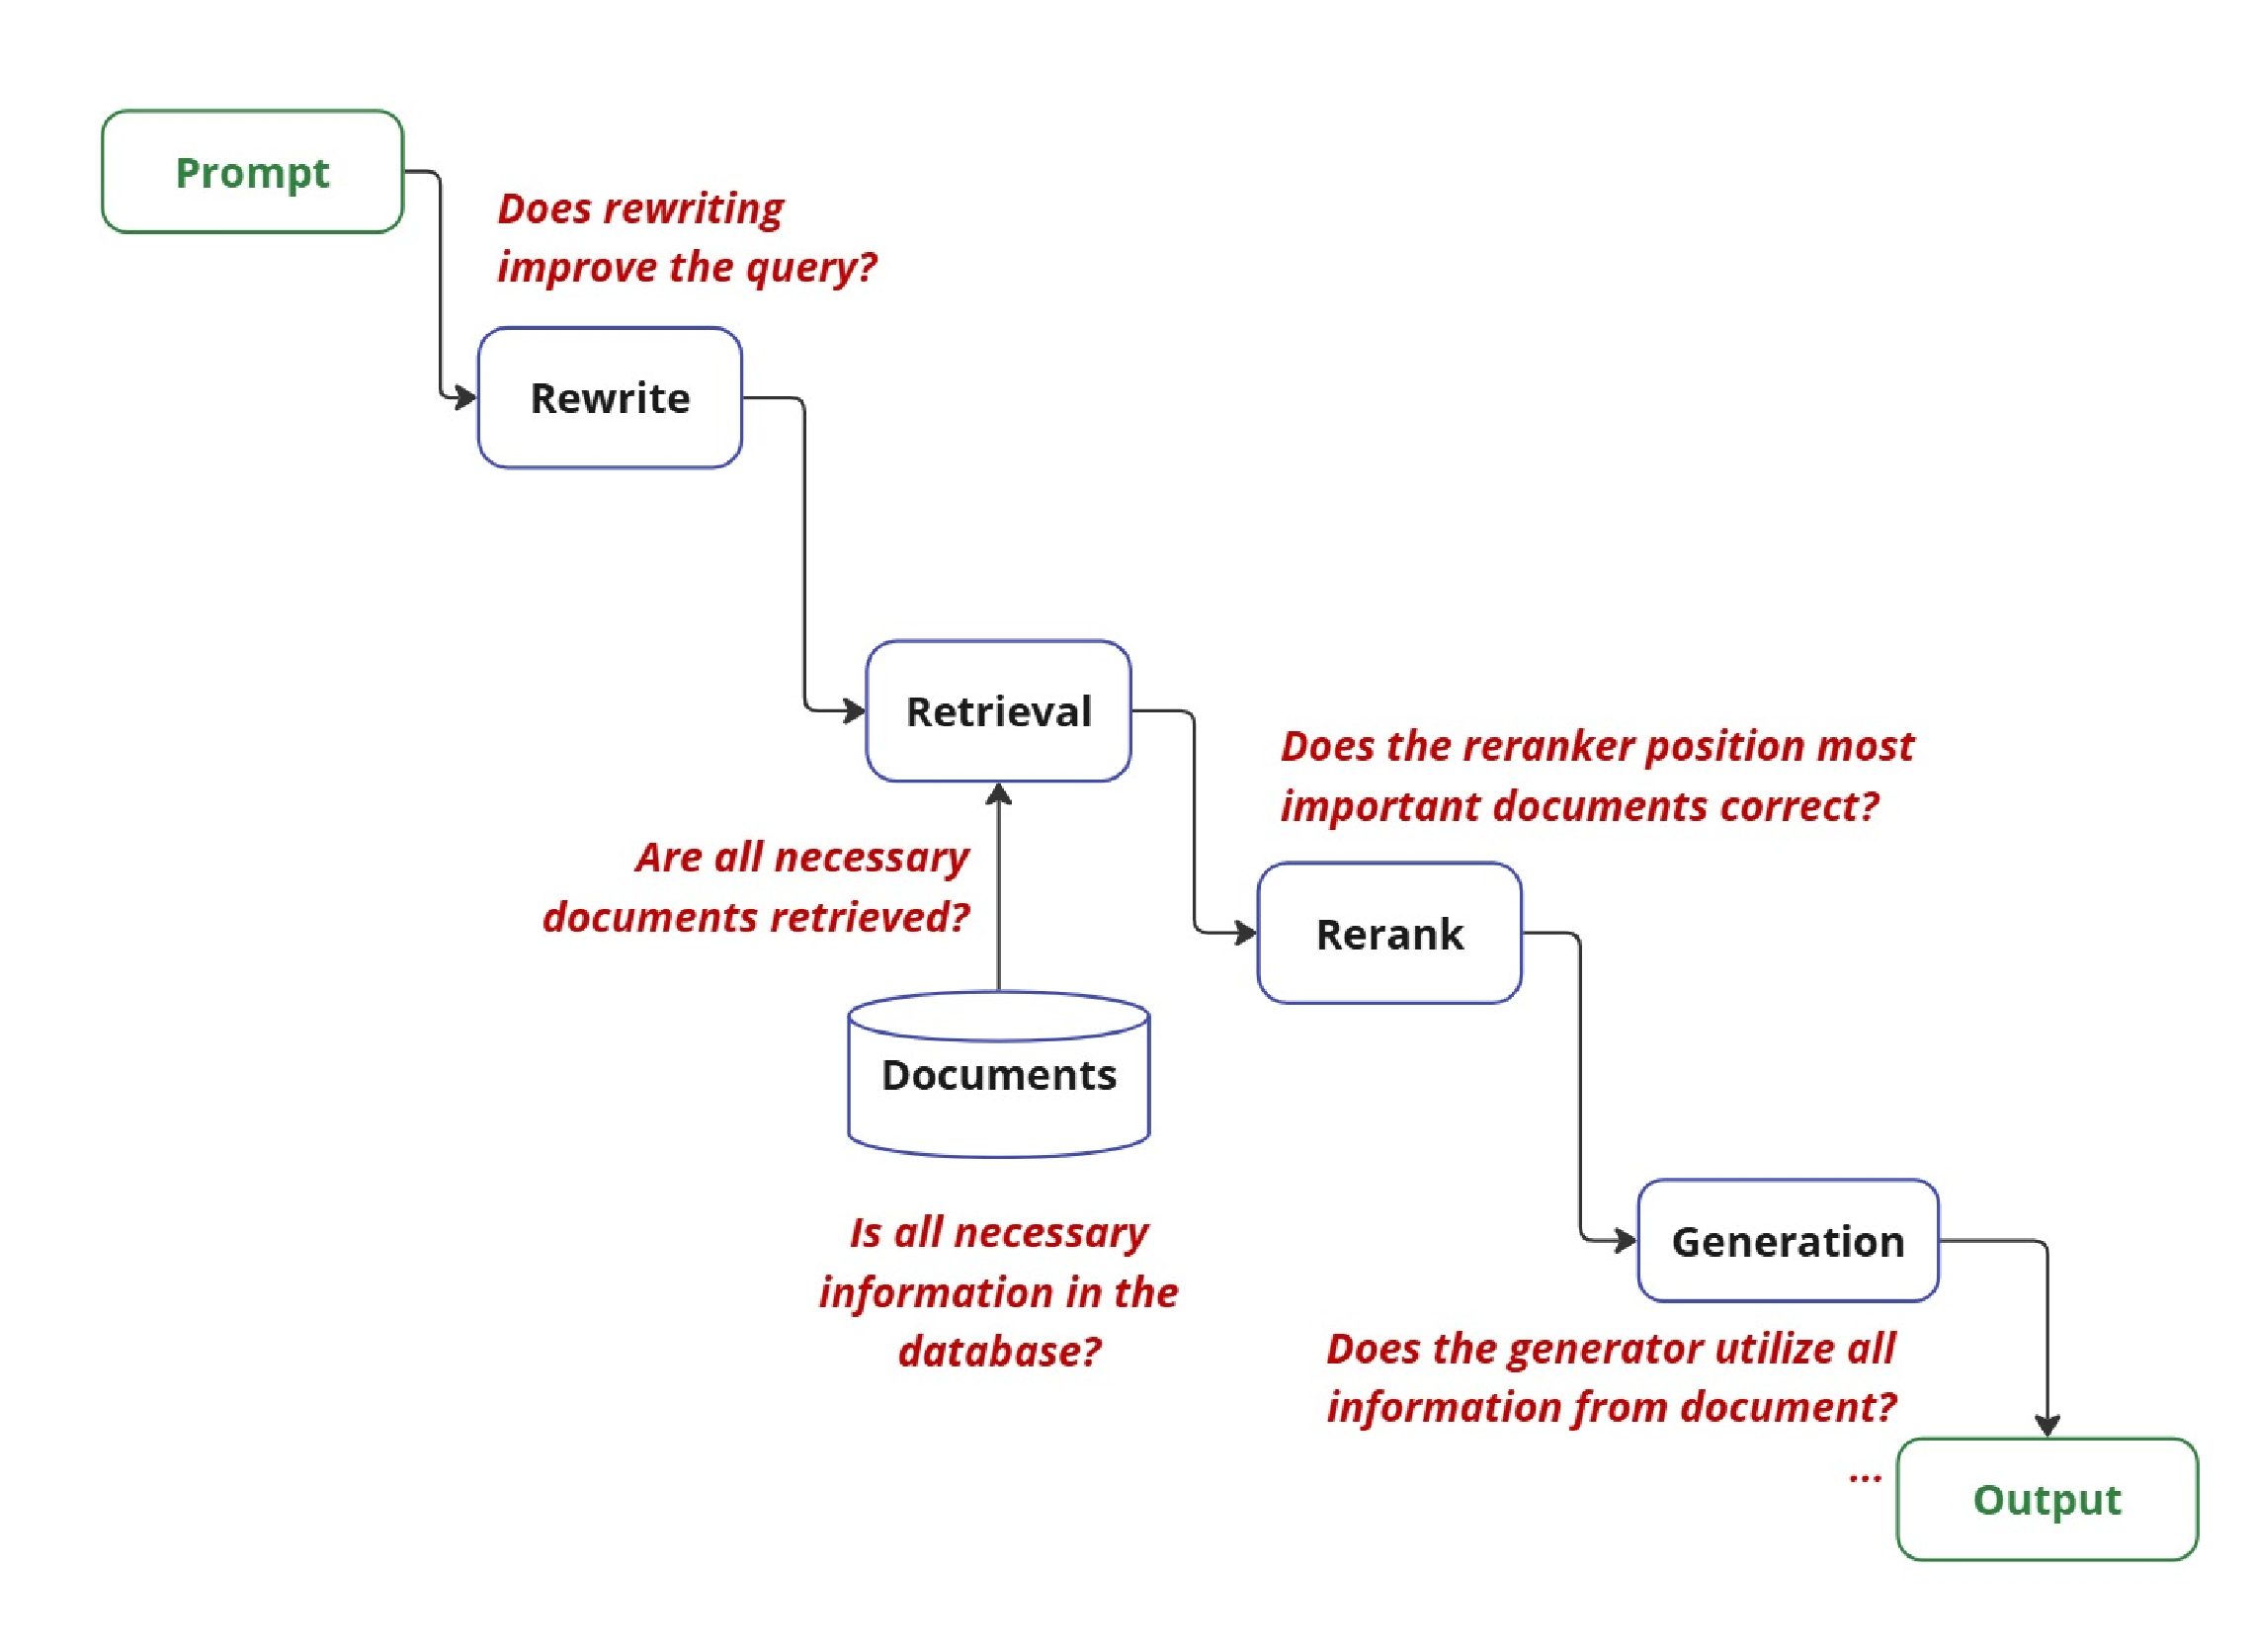
\includegraphics[width=\textwidth]{images/FailurePointExamples.pdf}
  \caption{A RAG pipeline with one failure example for each used component.}
  \label{fig:failures}
\end{figure}

\subsection{End-to-End Evaluation}

We define end-to-end evaluation as metrics that use the system's input query and its final output, comparing this output against a ground-truth reference to determine correctness. Evaluations that assess intermediate steps, such as retrieval performance or the generator's ability to utilize provided context, are considered component-level evaluations and are distinct from the end-to-end perspective discussed here. In this thesis, our focus is primarily on classification tasks; therefore, the end-to-end metrics employed are limited to those suitable for classification.

{\renewcommand{\arraystretch}{1.5}%
\begin{table}
  \centering
 \begin{tabular}{|l|l|}
  \hline
  \textbf{Metric} & \textbf{Formula / Description} \\[3pt]
  \hline Accuracy & $\frac{TP + TN}{TP + TN + FP + FN}$\\[5pt]
  \hline Precision & $\frac{TP}{TP + FP}$\\[5pt]
  \hline Recall & $\frac{TP}{TP + FN}$\\[2pt]
  \hline F1-Score & $2 \times \frac{Precision \times Recall}{Precision + Recall}$\\[2pt]
  \hline Matthews Correlation & $\frac{TP \times TN - FP \times FN}{\sqrt{(TP + FP)(TP + FN)(TN + FP)(TN + FN)}}$\\Coefficient & \\[2pt]
  \hline False-Positive Rate & $\frac{FP}{FP + TN}$\\[2pt]
  \hline False-Negative Rate & $\frac{FN}{FN + TP}$\\[2pt]
  \hline
 \end{tabular}
 \caption{Typical classification metrics used for experiments involving RAGs or LLMs\cite{Hou.8212023,Zeng.28.03.2024}.}
 \label{table:classification_metrics}
\end{table}}

In stark contrast to evaluating open-ended generative tasks, classification tasks benefit from well-established metrics and evaluation methods. Table \ref{table:classification_metrics} presents commonly used classification metrics relevant for RAG and LLM experimentation \cite{Hou.8212023,Zeng.28.03.2024}.

Meaningful end-to-end evaluation requires researchers to establish \textit{baselines} for their experiments. Baselines make results interpretable by providing essential points of comparison. Therefore, this framework implements two default baselines used when initiating an experiment. The first baseline consists solely of a standalone LLM answering the query without retrieval. The second is a naive RAG system employing BM25 retrieval with data from the predefined corpus (a simple retrieve-read pipeline, cf. section \ref{sec:naive_rags}). The standalone LLM baseline helps justify the complexity overhead of implementing a RAG system; if an evaluated RAG system cannot surpass the performance of the LLM baseline, a simpler approach might be preferable. Advanced RAG systems often involve more components, potentially leading to longer computation times and increased costs. Outperforming the naive RAG baseline demonstrates the value added by the more advanced RAG configuration beyond simple keyword retrieval.

\begin{figure}[h]
  \centering
  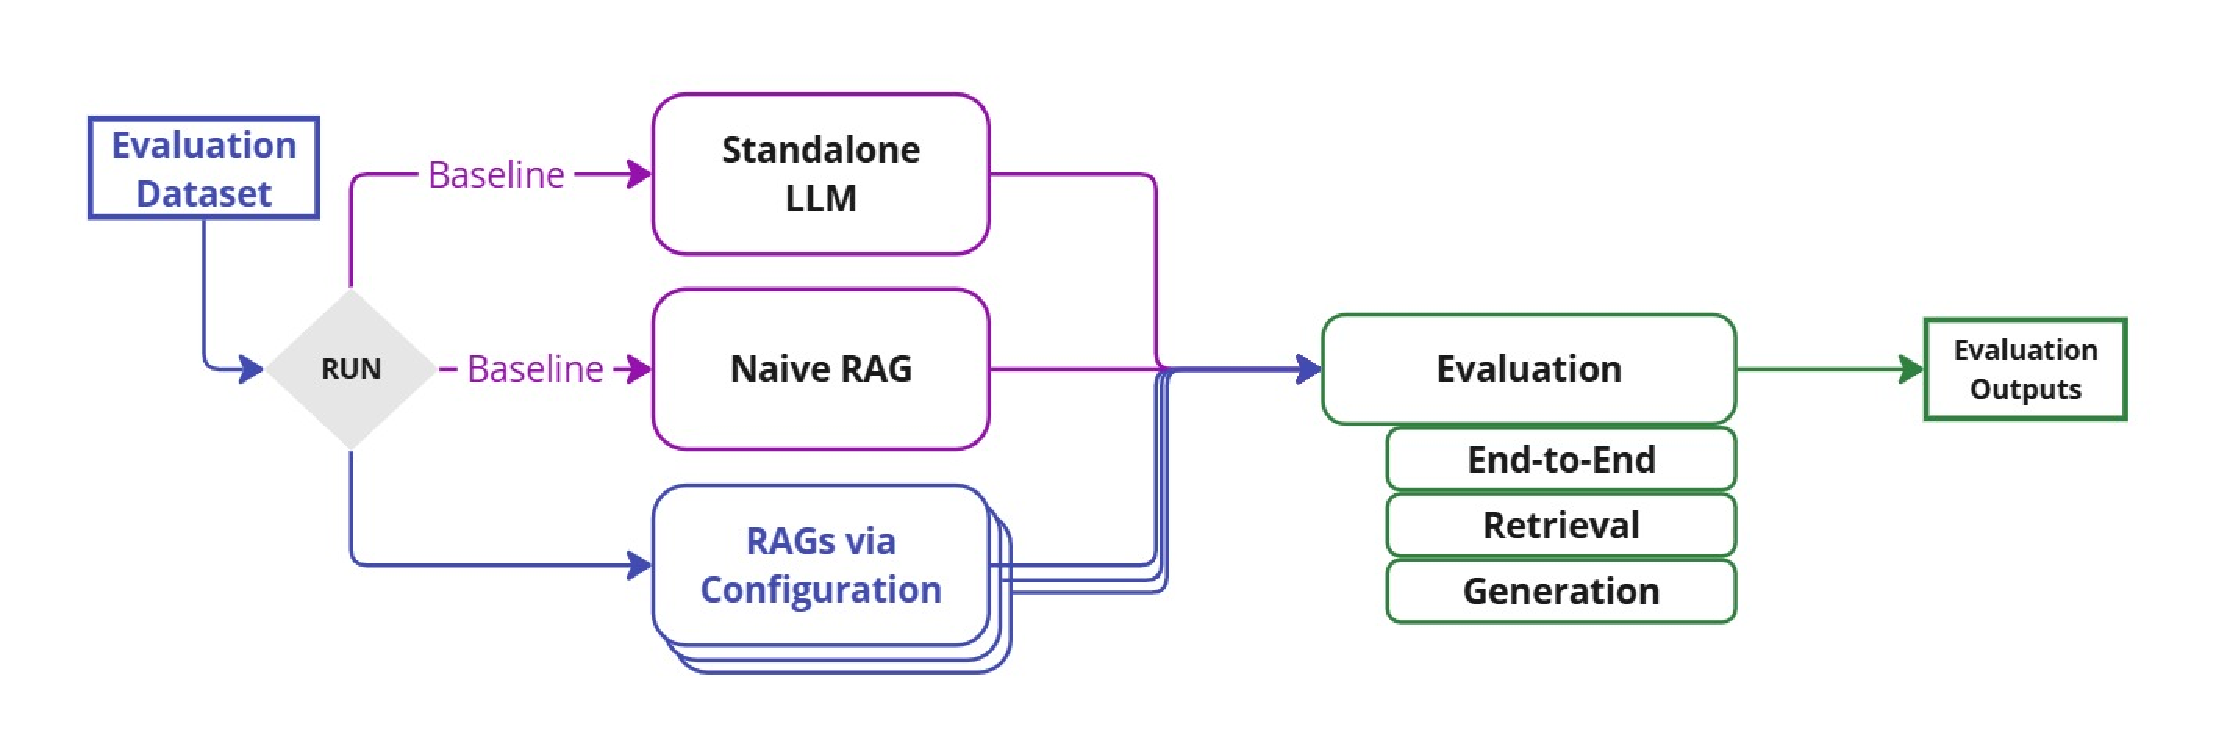
\includegraphics[width=\textwidth]{images/FrameworkBaselines.pdf}
  \caption{Framework Overview: Researchers define configuration files for RAG variations, which are evaluated against the standalone LLM and naive RAG baselines using end-to-end metrics.}
  \label{fig:framework-baselines}
\end{figure}
% \cite{Ru.15.08.2024.} Eventhough all components of a RAG-system affect its overall performance, there are ones that can not be evaluated directly.  \\

Figure \ref{fig:framework-baselines} illustrates the state of our framework as defined thus far, clarifying our approach. It depicts the process where evaluation data is used to compute metrics for both the defined baselines and the RAG configurations under test, performing both end-to-end and component-wise (retrieval and generation) evaluations. The following section details the component evaluation methodology employed in our framework.

\subsection{Component Evaluation}

Component evaluation is necessary to detect performance bottlenecks or issues introduced by individual components or problematic interactions between them \cite{Salemi.2024}. In Figure \ref{fig:failures}, we presented a few examples of such failures. While illustrative, this is far from an exhaustive list of potential failure points in a complex RAG system. We argue that potentially *all* components, no matter how seemingly small their impact, can contribute significantly to the overall system's failure rate. Therefore, ideally, it would be necessary to evaluate them all component-wise.

However, current literature on component evaluation primarily focuses on the core retrieval and generation (\textit{read}) stages. Furthermore, we want to emphasize that evaluating components in complete isolation from others is often impractical. If, for example, one wished to evaluate the generator component independently of the retrieval step, it would require providing a ground-truth dataset of ideal retrieved contexts for each query. This might be feasible for simple scenarios requiring only a single, easily identifiable document chunk (e.g., a sentence providing a direct answer). Yet, real-world scenarios frequently involve more complex cases, such as ambiguous queries, multifaceted questions requiring information synthesis, or queries that do not require retrieval at all \cite{Huang.2023}. Furthermore, if the researcher modifies the chunking strategy (e.g., size or technique), the ground-truth contexts would need to be recreated, as the previously selected chunks might no longer exist (cf. section \ref{sec:advanced_rags}).

Considering other components besides the retriever, such as query rewriters or document rerankers, establishing ground-truth data becomes even more problematic. The purpose of rewriting a query, for instance, is often to improve subsequent retrieval performance. Thus, its effectiveness is inherently dependent on the specific retriever used and cannot easily be assessed against fixed, retriever-agnostic ground-truth examples in an evaluation dataset.

Given these challenges, the primary purpose of component evaluation shifts towards identifying weaknesses within the RAG pipeline rather than achieving perfect isolated assessment. It is often more feasible to evaluate the RAG system using only the initial inputs and final ground-truth answers for end-to-end metrics, while employing non-deterministic LLM-as-a-Judge methods for assessing intermediate steps where appropriate. The LLM-as-a-Judge approach involves using a powerful LLM (often significantly larger or specifically trained for evaluation) to assess the quality of intermediate outputs (like retrieved context relevance) or final responses \cite{Chiang.2023}. Instead of relying solely on numerical metrics, the judge LLM provides qualitative assessments or scores based on predefined criteria.

Relying primarily on system input and final ground-truth datasets for evaluation offers significant time savings compared to creating extensive intermediate ground truths. However, detailed failure analysis to pinpoint the root cause of errors still necessitates tracing individual pipeline executions, which we utilize in this framework with Langfuse. The following sections detail our approach to evaluating the key retrieval and generation blocks using a combination of these techniques.

\paragraph{Retrieve}
Evaluating the retrieval component is arguably one of the most challenging aspects of RAG assessment for several reasons. First, retrieving more documents does not necessarily imply better final results, and it is often unclear which specific set of documents will best enable the generator to produce the optimal answer \cite{Jin.5222024}. Second, real-world indexed corpora often contain redundant and contradictory information \cite{Yu.2024}. Third, some queries require retrieving diverse perspectives on a topic, highlighting various considerations. Fourth, the quality of the input query itself significantly affects retrieval performance; queries can be overly complex or ambiguous, or may not even require retrieval, potentially leading to generator hallucinations if irrelevant or misleading context is fetched \cite{Huang.2023, Mallen.20.12.2022}.

While retrieved documents can often be assessed in a binary fashion (relevant/irrelevant), allowing for metrics based on \textit{True/False Positives/Negatives}, simple metrics like precision and recall are often not sufficiently sensitive to capture nuanced differences in retrieval quality \cite{Yu.2024}. There is a clear need for evaluation techniques that also consider the ranking of retrieved documents.

Furthermore, significant limitations exist when working with ground-truth data for retrieval evaluation. Defining a definitive ground-truth set of relevant context documents for a given query can be ambiguous and challenging even for human experts, although LLM-as-a-Judge models have shown high correlation with human judgments in this area \cite{Chiang.2023}. Compounding this issue is the dynamic nature of chunking during reconfiguration. Every time a chunking technique or parameter is altered, the resulting indexed documents change, necessitating the recreation of ground-truth retrieval datasets. This poses a significant bottleneck for rapid development cycles, yet tuning chunking strategies is crucial. Therefore, to maintain flexibility and speed, this framework focuses primarily on LLM-as-a-Judge evaluation for the retrieval component, particularly enabling effective chunking parameter tuning.

We utilize a metric named \textit{Context Relevance} (akin to \textit{Context Precision} in other frameworks) which employs an LLM-as-a-Judge. This metric assesses the relevance of each retrieved document concerning the input query. A binary approach is typically adopted: the LLM-as-a-Judge determines if a document contains statements relevant to the query. If yes, the document scores 1 (relevant); otherwise, it scores 0 (irrelevant). Haystack's `ContextRelevanceEvaluator` \cite{Pietsch_Haystack_the_end-to-end_2019}, for instance, implements such a binary assessment. The final \textit{Context Relevance} score is the mean of these binary scores across all retrieved documents for a query (and typically averaged over all queries in the dataset), yielding a score analogous to Mean Precision. While some frameworks like RAGAS might infer retrieval quality from the generated response, our approach, similar to Haystack's, directly evaluates the relevance of the retrieved documents themselves via the LLM-as-a-Judge.

Recognizing that simple relevance counts (like Context Relevance/Precision) do not capture ranking quality, we also implement \textit{Mean Average Precision at K (MAP@K)} to offer a complementary, rank-aware perspective. MAP@K evaluates whether relevant documents are ranked higher in the retrieved list \cite{EvidentlyAIInc..25.02.2025}. 

$$MAP@K=\frac{1}{|Q|}\sum_{q=1}^{|Q|}AP@K$$
$$AP@K=\frac{1}{N}\sum_{k=1}^{K}Precision(k) \cdot rel(k)$$
\begin{itemize}
  \item $|Q|$ is the total number of queries in the evaluation set.
  \item $q$ represents a specific query
  \item $AP@K$ is the Average Precision at K for a specific query.
  \item $N$ is the total number of relevant items for a particular query.
  \item $K$ is the number of top documents being evaluated.
  \item $k$ represents a specific position in the ranked list of retrieved documents.
  \item $Precision(k)$ is the precision calculated at position $k$, defined as the number of relevant items among the top $k$ items divided by $k$.
  \item $rel(k)$ equals 1 if the item at position $k$ is relevant and 0 otherwise.
\end{itemize}

The formula presented is the standard definition of MAP@K \cite{Lin.13.10.2020}. While in some traditional information retrieval scenarios K might be set very high, this can be computationally expensive and may conflict with the goal of providing concise context. Therefore, we calculate MAP@K based on the actual number of documents retrieved (i.e., the system's configured \textit{Top-K} parameter). \textit{Context Relevance} measures overall retrieval quality by focusing on the proportion of relevant items, while \textit{MAP@K} specifically assesses the ranking quality within the retrieved set. A low \textit{Context Relevance} score alongside a high \textit{MAP@K} score might indicate that while relevant documents are found and ranked well, too many irrelevant documents are also being retrieved, suggesting the \textit{Top-K} parameter could potentially be reduced. Conversely, a low \textit{MAP@K} suggests the retrieval/ranking mechanism itself needs adjustment, as irrelevant documents frequently appear high in the results list.

\begin{figure}
  \centering
  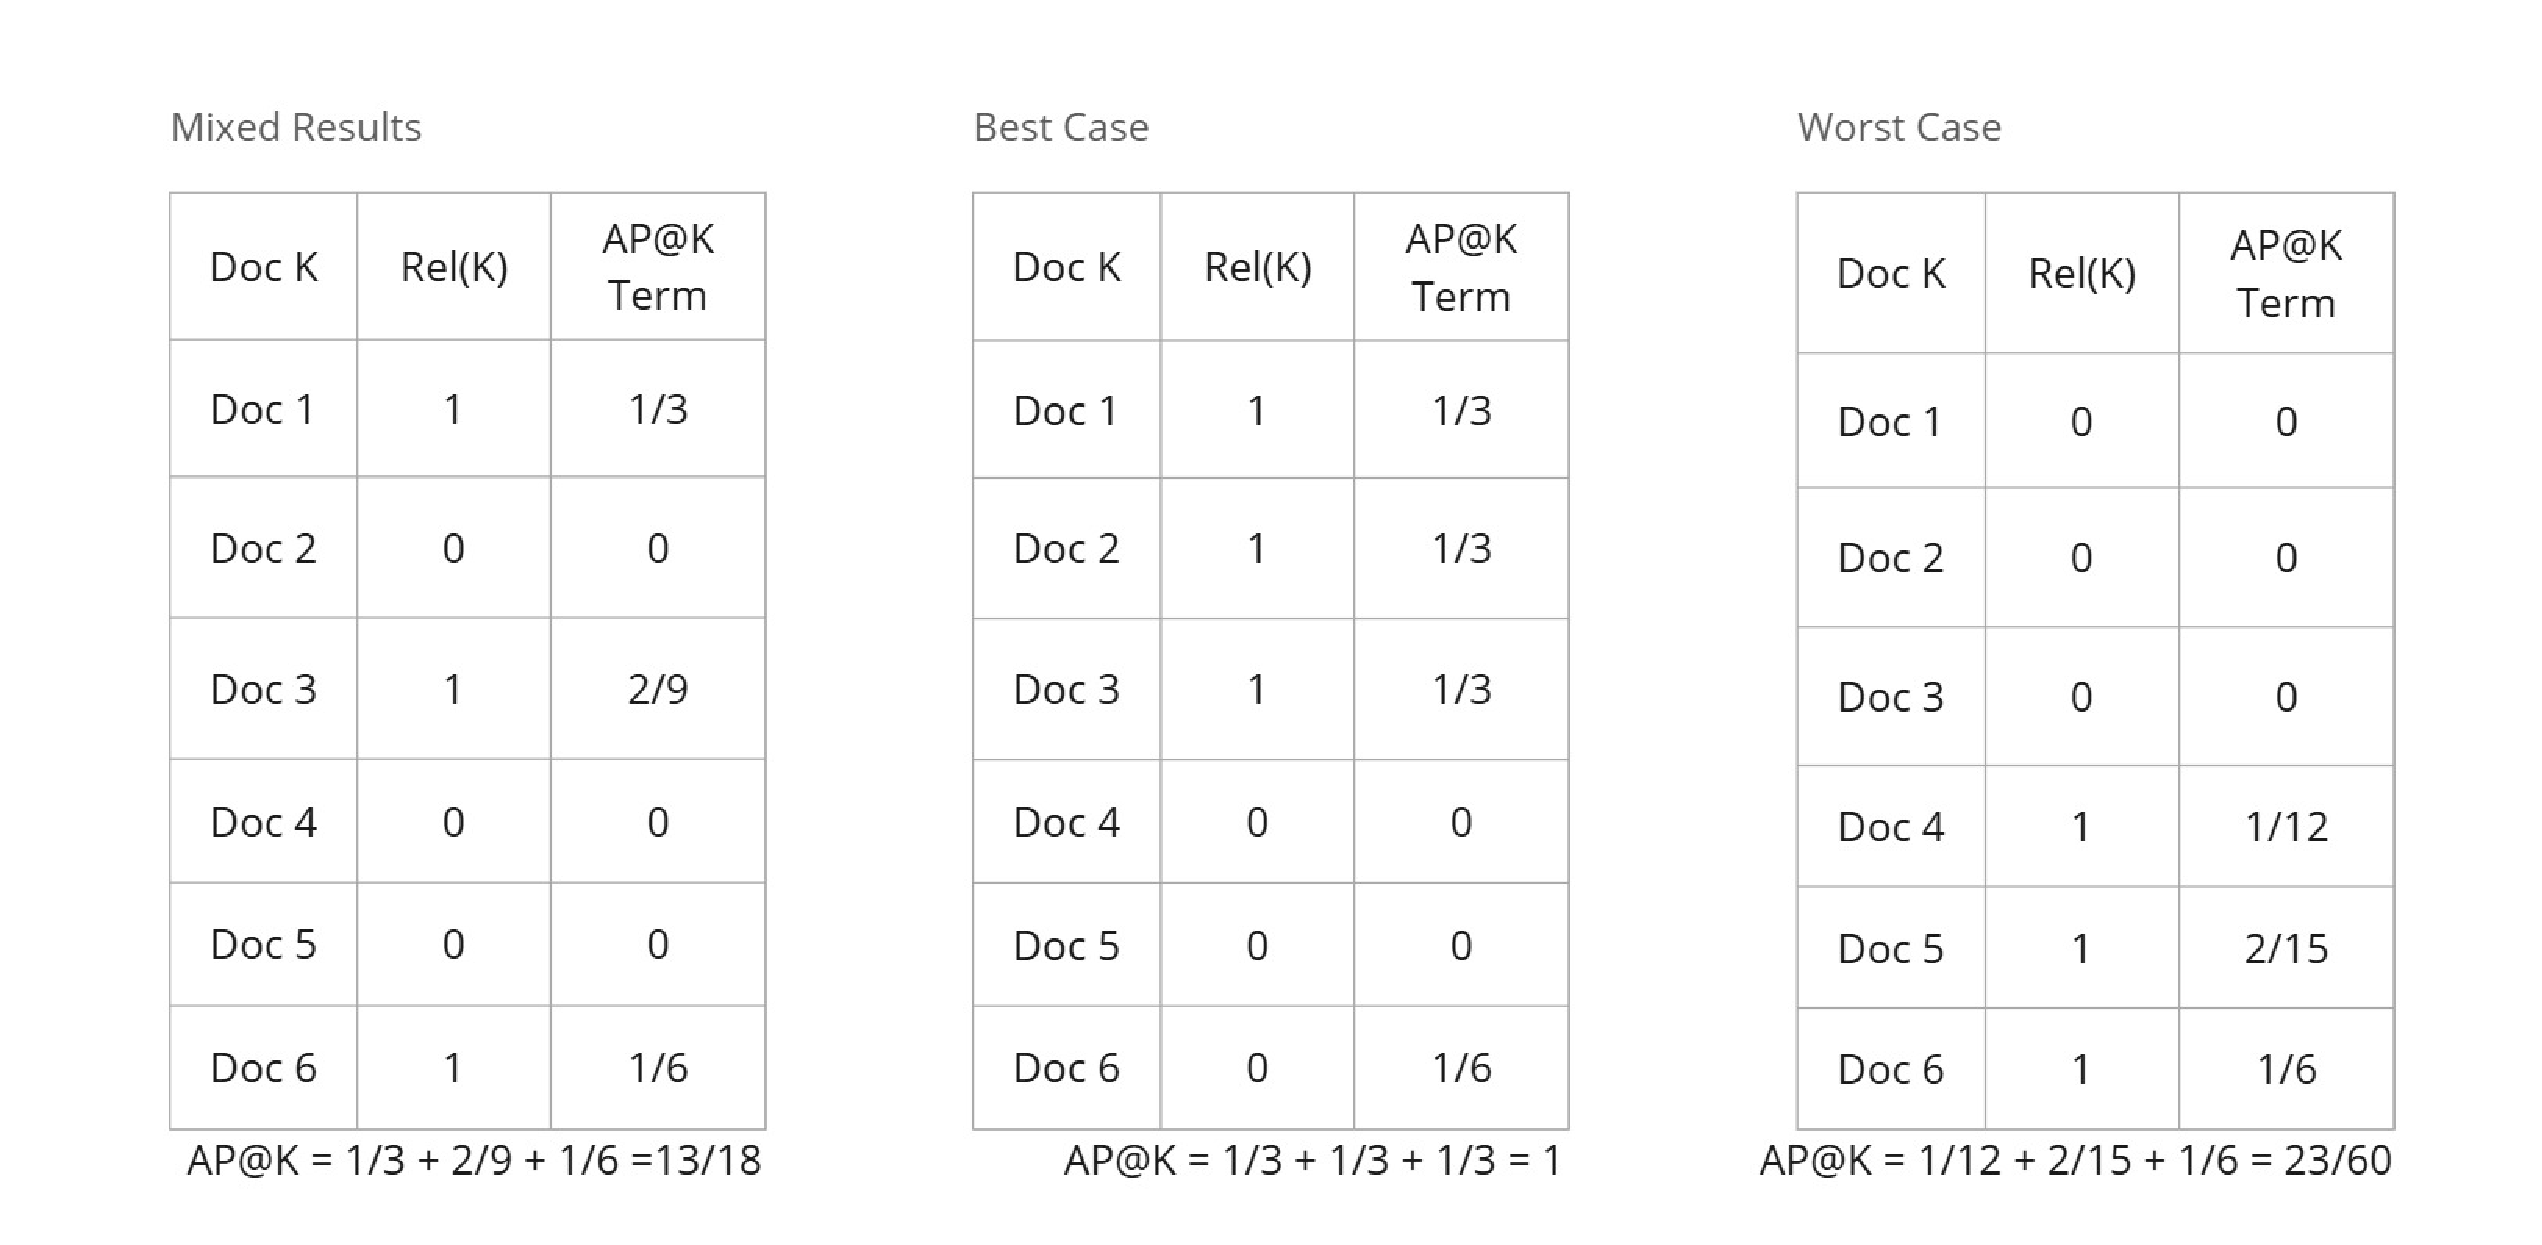
\includegraphics[width=\textwidth]{images/APatK.pdf}
  \caption{This is an example for AP@K metric for one query. At each retrieved document relevance and precision of the first to K-th document will be averaged through all retrieved documents.}
  \label{fig:APatK}
\end{figure}


\paragraph{Generators}
Generators in RAG systems, typically based on transformer architectures, were not initially designed primarily for classification tasks. Consequently, ensuring their outputs adhere to specific, desired formats (e.g., producing only \textit{valid} or \textit{invalid}) is an important preliminary check. This necessitates a metric or process to evaluate the generator's ability to follow formatting instructions; we refer to this as \textit{format validation}. However, a significant challenge arises when evaluating generators solely on classification accuracy: simple binary outputs (\textit{True/False}, \textit{Valid/Invalid}) make it difficult, if not impossible, to directly assess crucial underlying aspects like whether the retrieved context was properly utilized or how relevant the generated answer is to the context.

Even when the final prediction is simply \textit{True} or \textit{False}, the underlying generation process involves varying degrees of context utilization and reasoning quality. Therefore, in this framework, we adopt a slightly modified output format for classification tasks to gain more insight. Instead of requiring the generator to produce *only* the binary label (e.g., \textit{0}/\textit{1}, \textit{valid}/\textit{invalid}, \textit{True}/\textit{False}), we prompt it to also output its reasoning *alongside* the classification verdict. The primary technical constraint is that the final answer label itself (e.g., the phrase \textit{'The answer is "True"'}) must be present in a predictable pattern within the output, allowing us to extract it reliably, for instance, using a regular expression for end-to-end metric calculation. The figure \ref{fig:answerreason} shows a simple example.

\begin{figure}
  \centering
  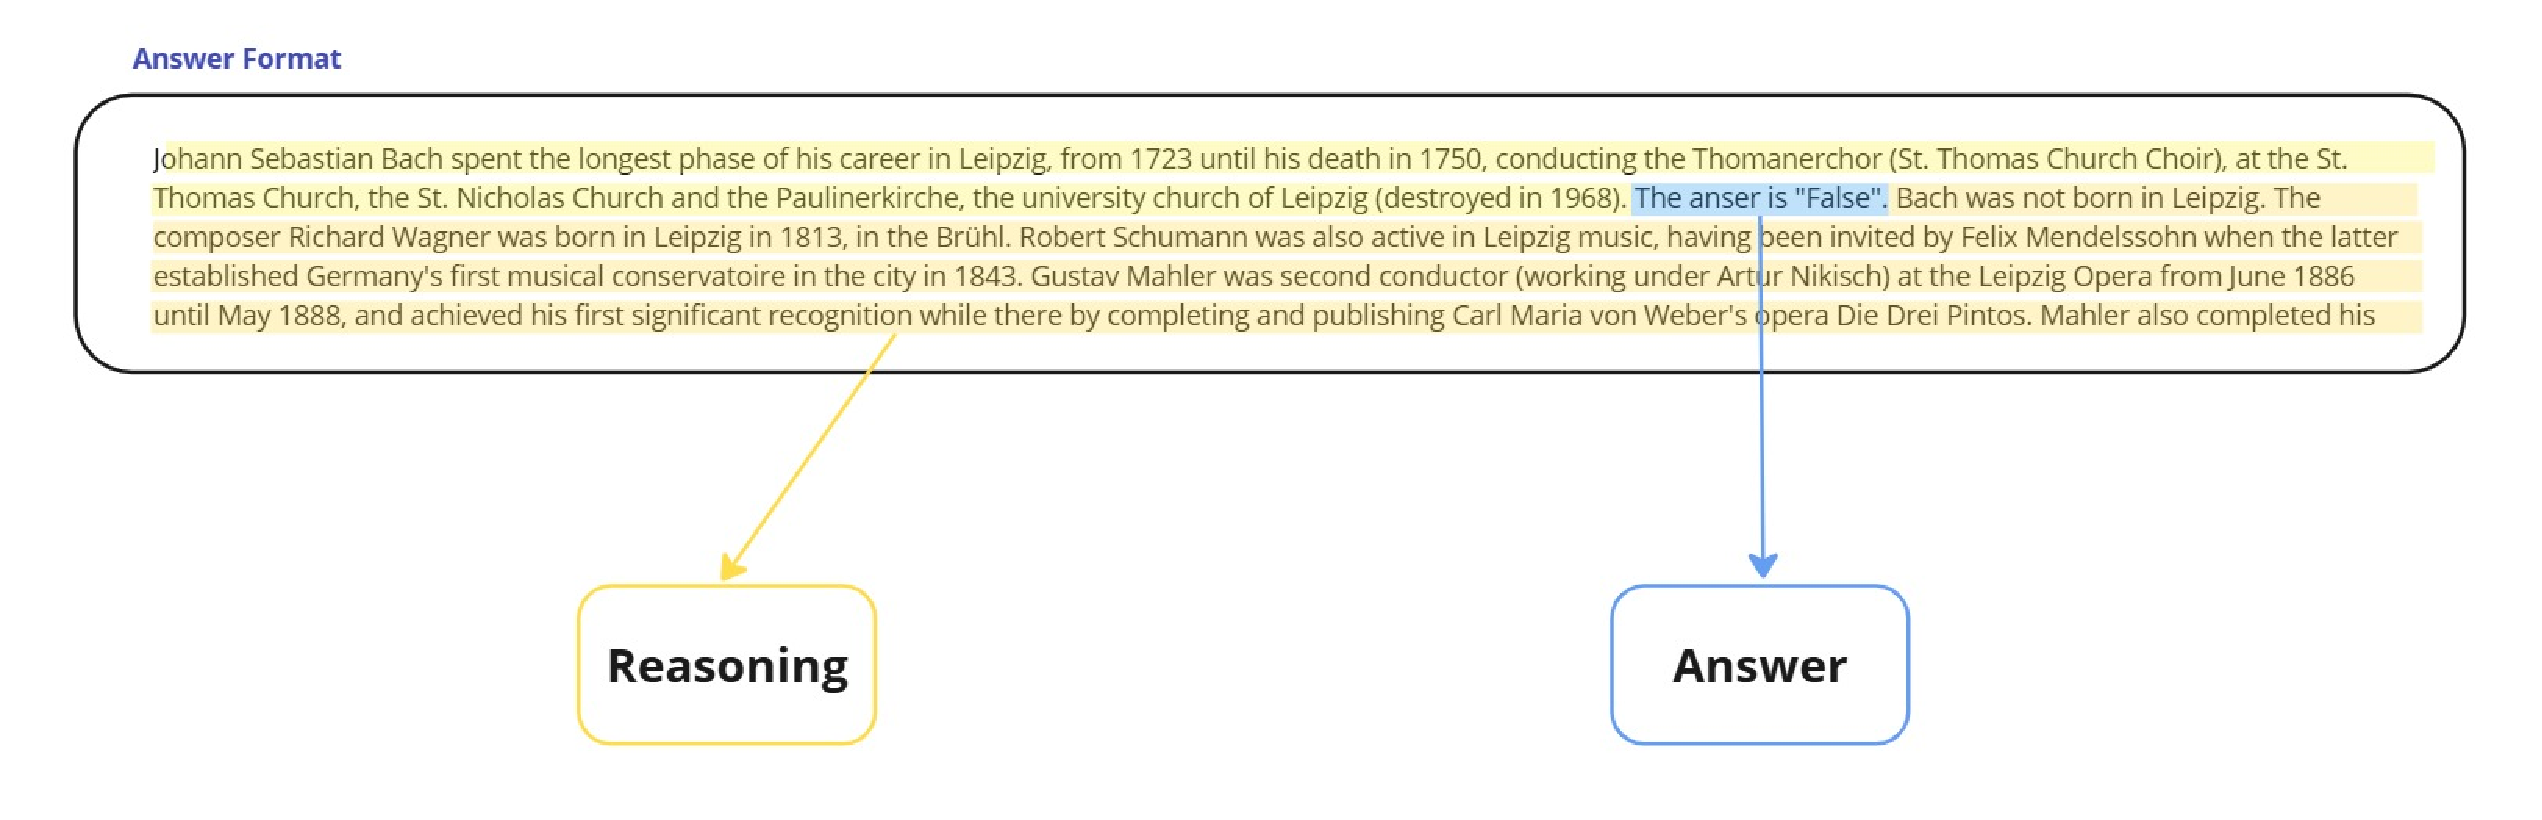
\includegraphics[width=\textwidth]{images/Answer-vs-Reasoning.pdf}
  \caption{This shows the answer of an generator and the final answer which we are using for binary classification.}
  \label{fig:answerreason}
\end{figure}

This has several positive side affects. First, we can measure the reasoning to assess context utilization or answer relevancy, which are important to debug the system. If the context of retrieval is not utilized enough, then we won't figure that out by analyzing binary classes. Second, we enable reasearchers to the current test-time compute paradigm shift for large language models or \textit{large reasoning models}. In practice, they use \textit{<think>...</think>} and use different search algorithms for the best reasoning path before these model answer the query. This leads to significantly better results.\cite{Xu.16.01.2025}


\subsection{Component Block Evaluation}

After evaluating component-wise, we need to evaluate other components, that are not assessable isolated too. In an advanced RAG such a component would be the rewriter. Rewriters try to synergize query to retrieval and context. Defining a performant rewriter depends on whether the RAG uses a sparse or a dense retrieval as he must either use relevant keywords or simulate semantic similarity. The second component from an advanced RAG system would be reranking. Both, reranker and generator have an great impact and interest in context utilization, the ability to build a coherent and correct answer based on actual facts from the retrieved context. Phenomena such as lost-in-the-middle have a significant affect on context utilization, but LLMs differ in this effect.\cite{Liu.06.07.2023} Therefore it might happen that the best reranker and generator regarding their component-wise performance lead to inferior context utilization results. The system needs to be model-agnostic for all components and researchers need rigorous testing of potential component blocks. 

\paragraph{How to evaluate such component blocks?}

\begin{figure}
  \centering
  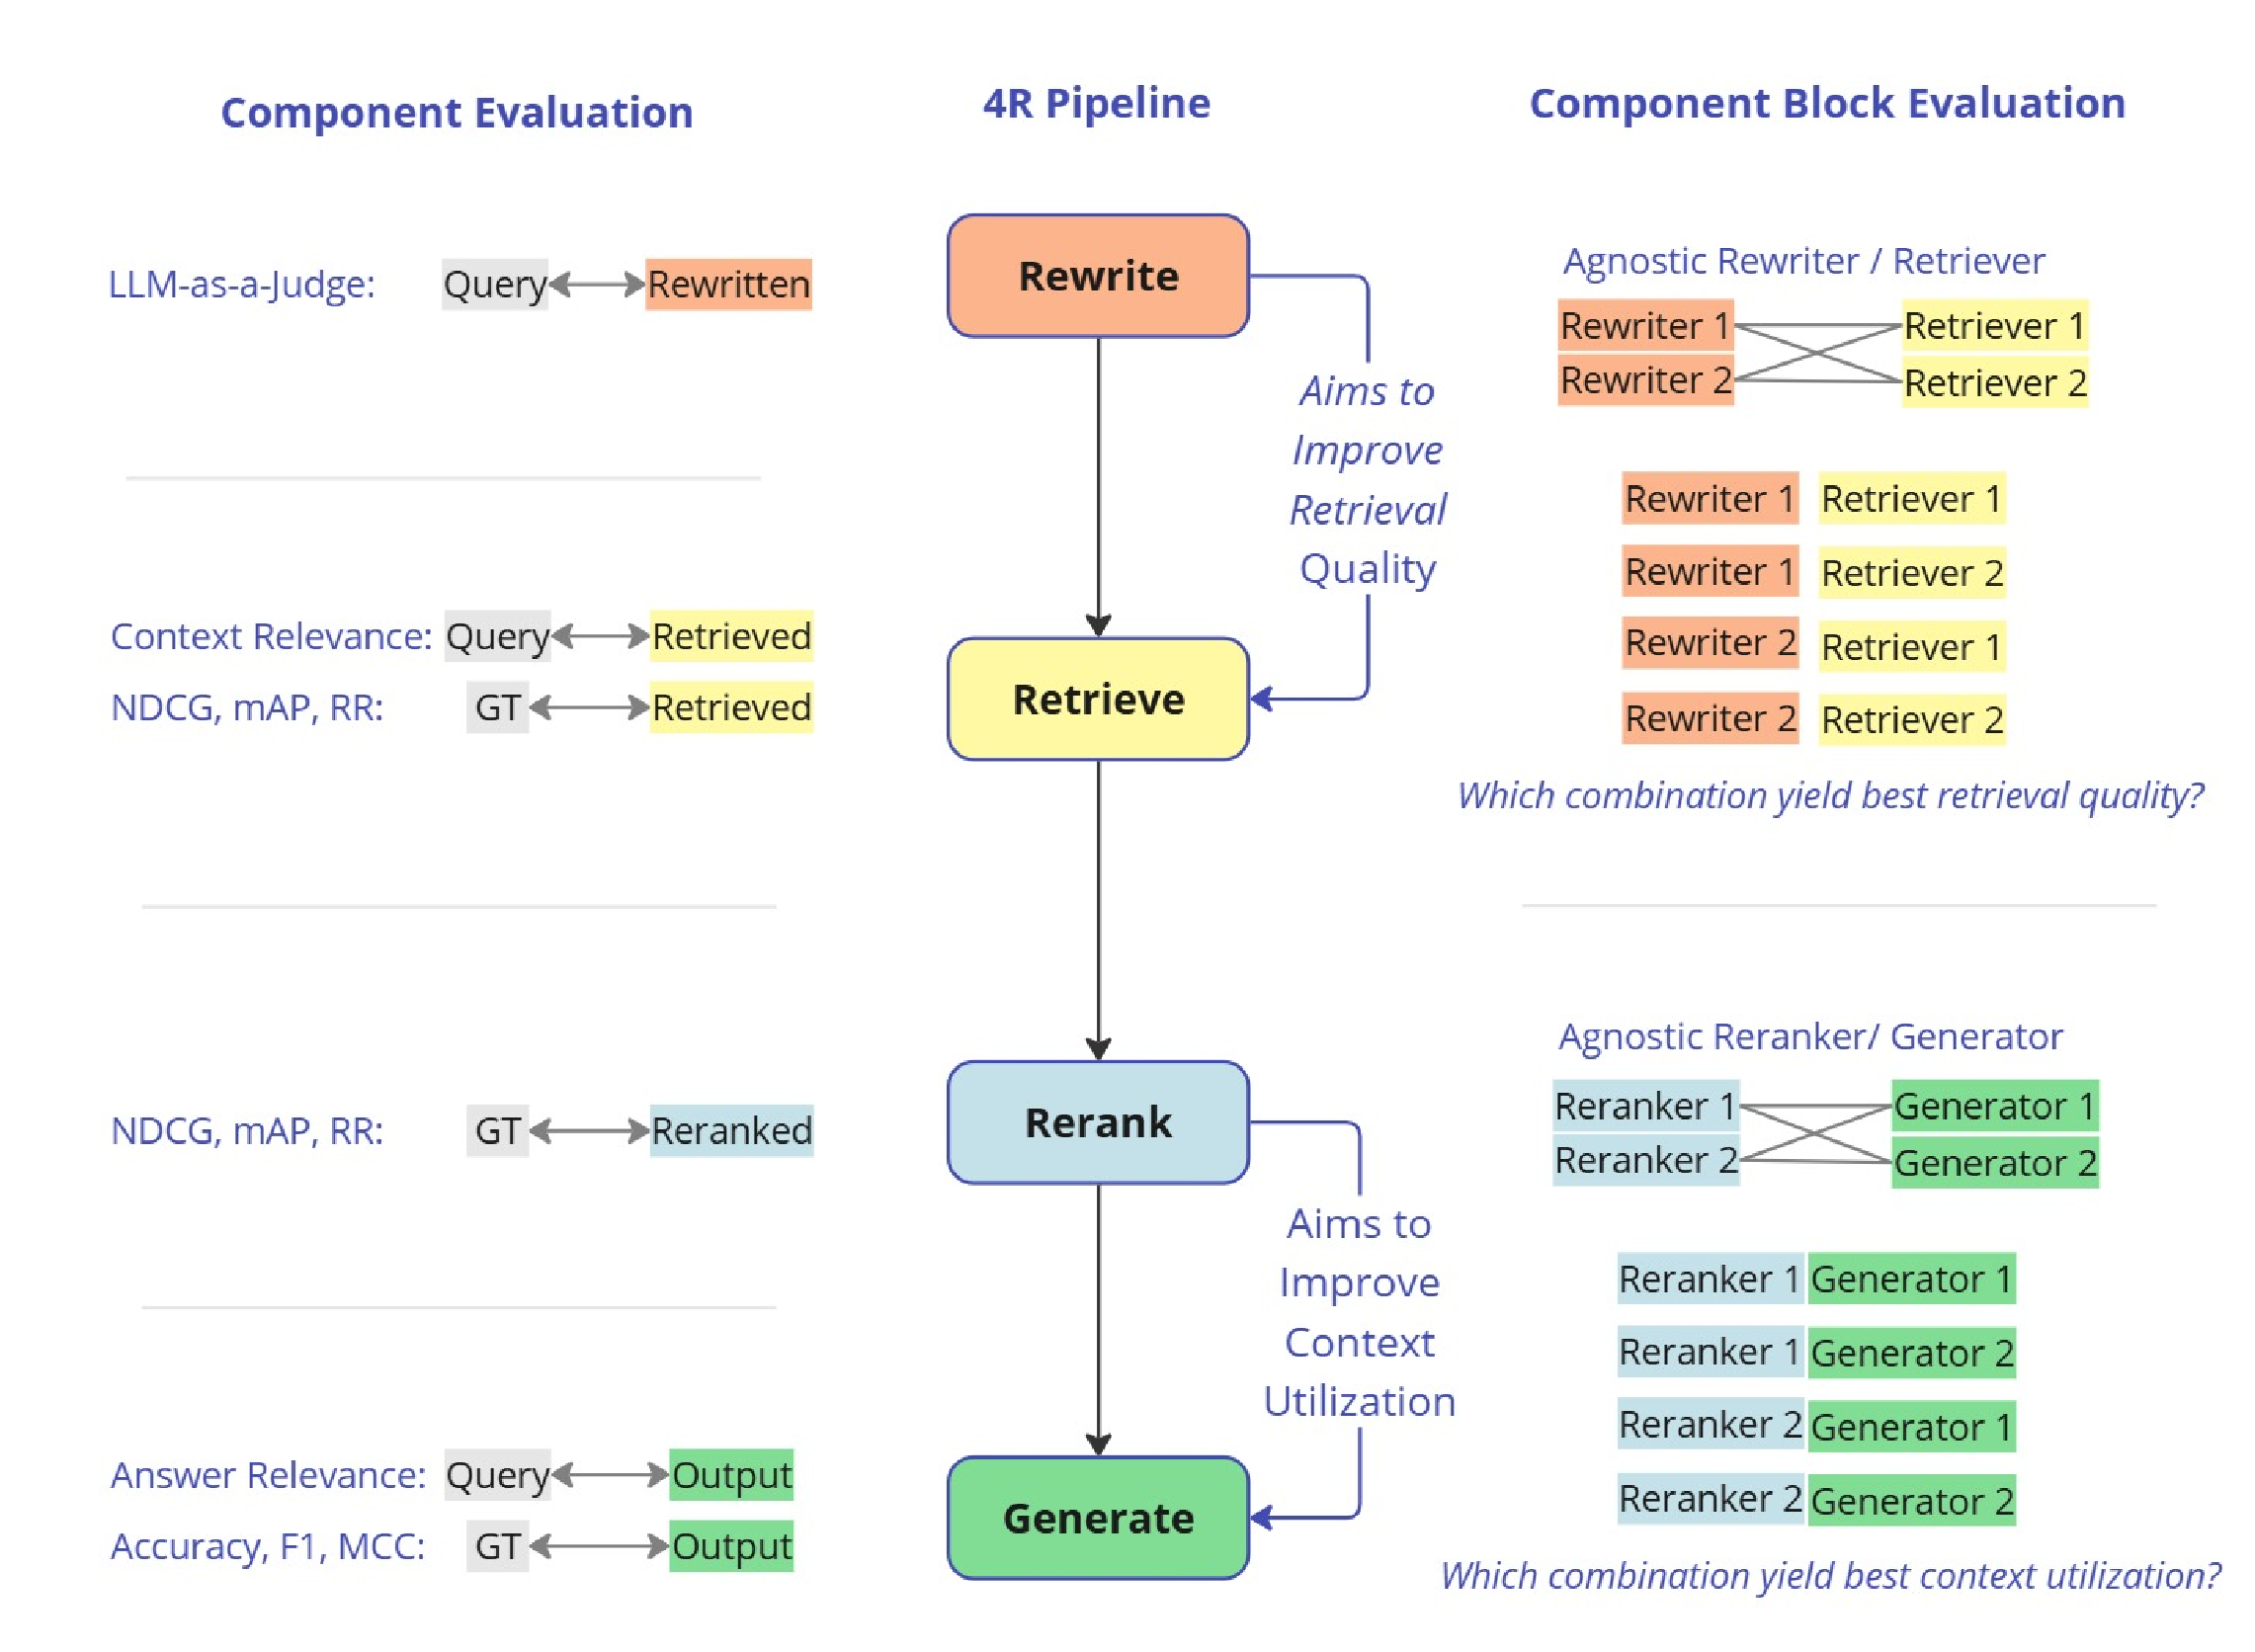
\includegraphics[width=\textwidth]{images/ComponentBlockEvaluation.pdf}
  \caption{Comparison of isolated component evaluation of each component and component block evaluation, where several components with the same goal are evaluated.}
  \label{fig:componentblockeval}
\end{figure}


We differentiate two major blocks - pre-retrieval and post-retrieval. Evaluating pre-retrieval component blocks such as rewriter is a derived task from the retrieval evaluation. The goal of pre-retrieval is to increase the retrieval quality so that the retriever finds all necessary documents or chunks for this task. Commonly used pre-retrieval techniques are query routing, query transformation and query expansion. Even in the ingestion stage, chunking, document selection and preprocessing steps are tuning parameters that influence retrieval results and its quality. 

Post-retrieval components such as reranker aim to improve the context utilization for the generator. The generator requires a curated and limited list of documents that serves its ability and query best. Second, reducing the Top-K parameter for retrievers might result in missing documents with required information. For that we use the same metrics as for the retriever. The additional step of reranking influences the overall performance and evaluating this component is important. 

Most components beside retriever and generator have no direct measurement,there they have to be evaluated by replacement and metrics of the component block. For example, the rewriter is evaluated by using similar components, different models or prompting techniques as rewriter-variations. Then the RAG runs through the evaluation by only changing those rewriter specific configurations. The resulting end-to-end or if applicable the resulting retrieval metrics decide which rewriter setting is better suited. This approach requires the researcher to try many different RAG variations for rigorous testing. In the next section we will introduce our appraoch for fast RAG development.

\section{Fast RAG Development}

\begin{figure}[b]
    \centering
    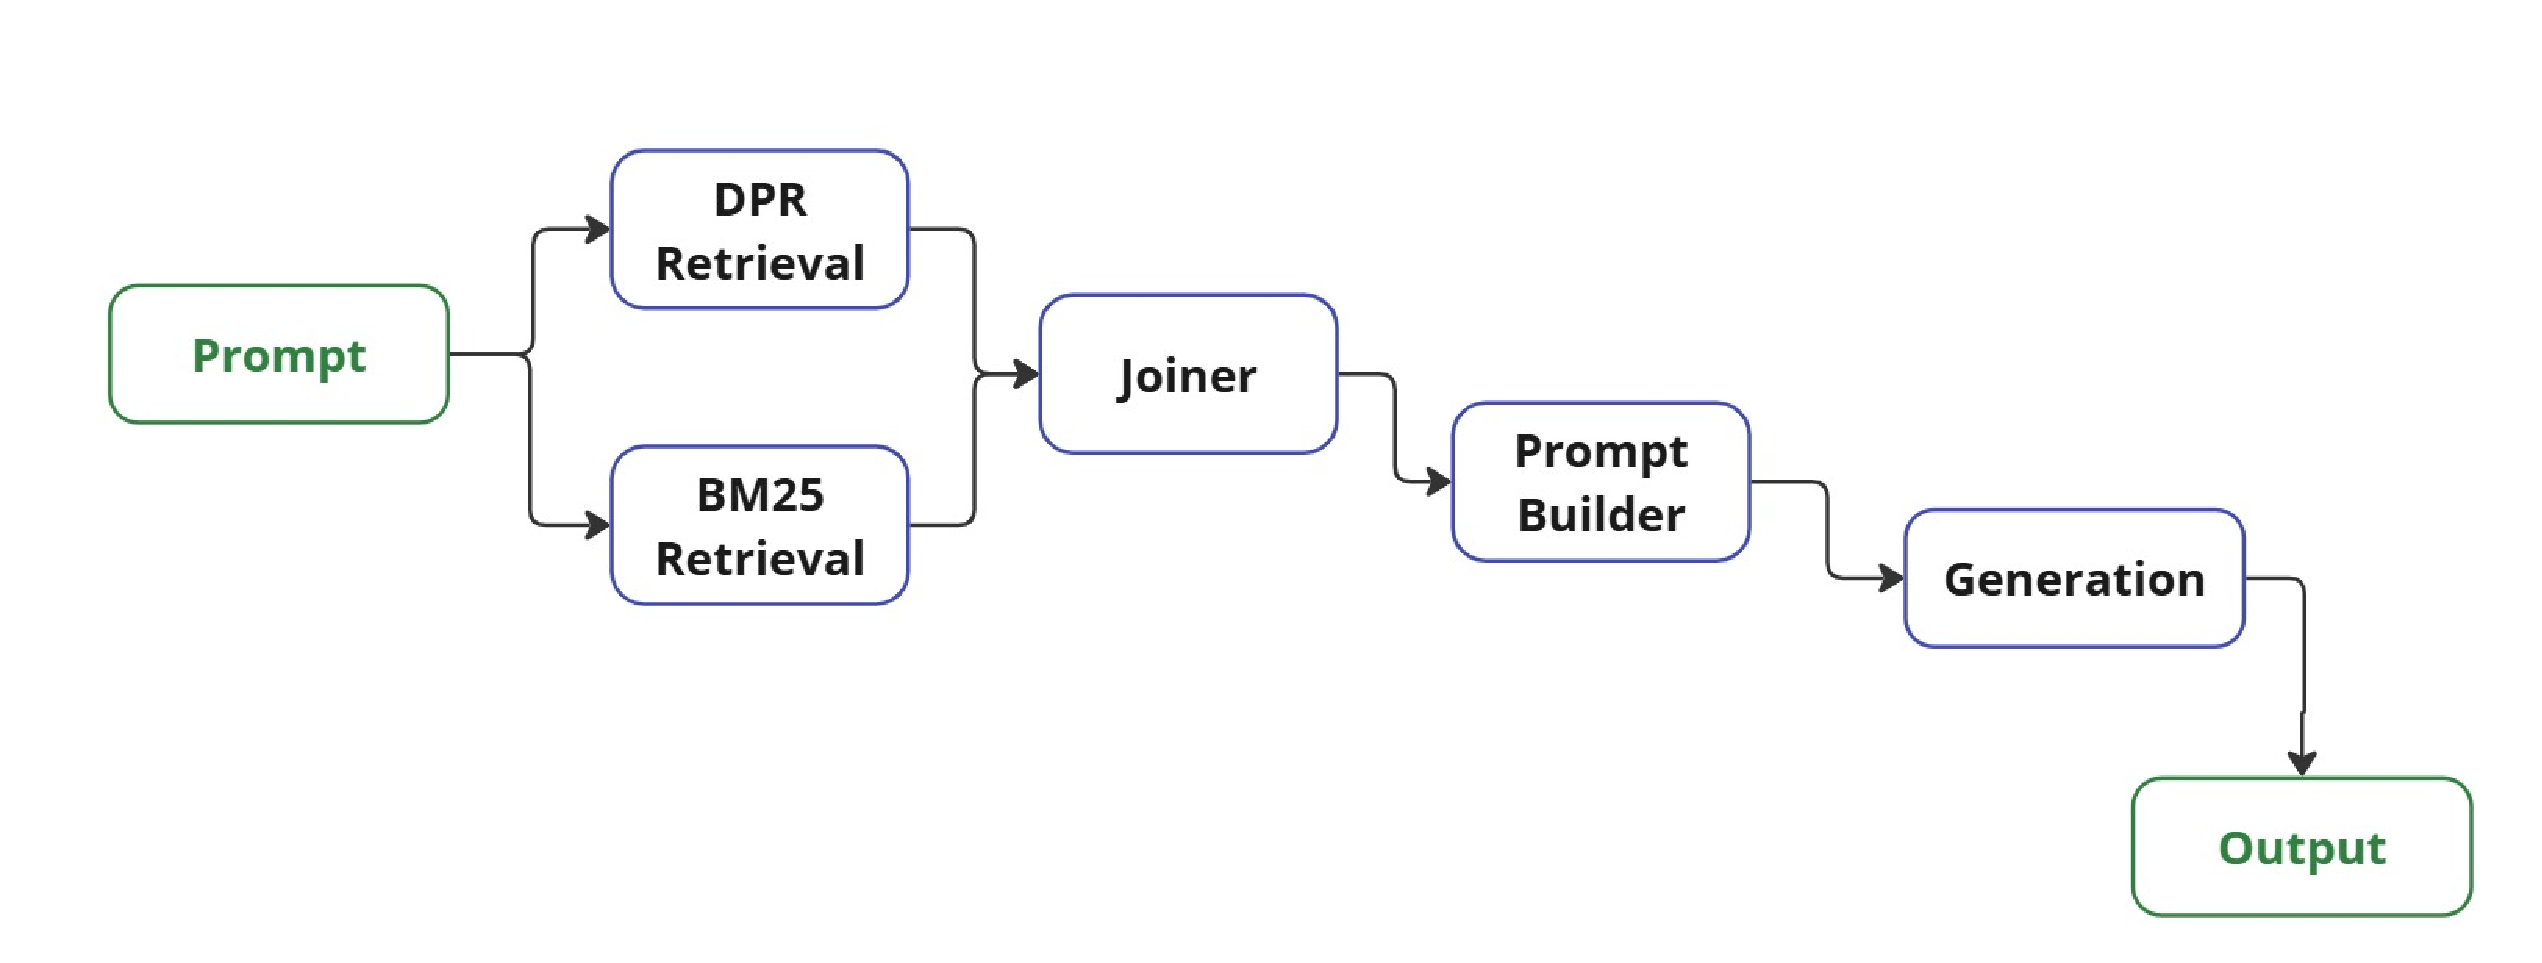
\includegraphics[width=\textwidth]{images/showcase-pipeline.pdf}
    \caption{A simple Retrieve-Read pipeline with both dense and sparse retrieval.}
    \label{fig:showcase}
\end{figure}

RAG systems have a lot of parameters that are not obvious to set. It is common as a researcher to have several reconfiguration phases till the RAG systems works sufficient. More reconfiguration phases lead logically to better results. Therefore Short feedback cycles and fast development make it possible to evaluate many configurations and short feedback cycles can lead to fast bottleneck improvements. This sections presents our considerations for offering fast RAG development.

There are several RAG development tools and frameworks. Highly used ones are Llama-Index\cite{Liu_LlamaIndex_2022}, Langchain\cite{Chase_LangChain_2022} and Haystack\cite{Pietsch_Haystack_the_end-to-end_2019}. All of them offer comparable functionality for building advanced RAG systems in modularized architecture as introduced by Gao et al.\cite{Gao.18.12.2023}. Haystack comes with custom components that enable new component technologies and does offer a functionality, where users can define a pipeline via a YAML-file. This enhances the reconfiguration of such systems, because instead of editing python files, there are just parameters in one YAML-file to be changed. This enhances the ability to report the methodologies of each experiment too. Instead of saving a python script or module for each configuration, only a YAML is stored that describes the tested RAG architecture fully. An example of this YAML definition can be seen in figure \ref{fig:showcase} and the YAML code below.

There are are more benefits for configuring via YAML files. First, we can copy existing RAG configurations easily. Second pipeline definitions can still be done in python, saving the afterwards into the YAML format. Lastly, Haystack develops an UI\cite{haystack-ui} for developing RAG system, that can be used to create such complex systems on a two-dimensional space.

\begin{minted}[
    frame=single,
    bgcolor=lightgray
  ]{yaml}
components:
  llm:
    init_parameters:
      api_base_url: null
      api_key:
        env_vars: OPENAI_API_KEY
      ...
  prompt_builder: ...
  bm25_retriever: ...
  embedding_retriever: ...
  joiner: ...
  text_embedder: ...
  docs_embedder: ...
  answer_builder: ...
connections:
- receiver: llm.prompt
  sender: prompt_builder.prompt
- ...
\end{minted}

While copying configuration files and adjusting parameters of it is more efficient then handling verbose python modules, we expanded haystacks core functionality for saving and loading YAML configurations with matrix notation.
We allow different parameters within a list and generate all possible combinations of that configuration. In the example below we can see 4 different combinations: ("gpt-4o-mini", 5), ("o3-mini", 5), ("gpt-4o-mini", 10) and ("o3-mini", 10). This ensures that the researcher can try and validate many different models or parameters and compare their impact on the overall performance.

\begin{minted}[
  frame=single,
  bgcolor=lightgray
]{yaml}
components:
  llm:
    init_parameters:
      model: ["gpt-4o-mini", "o3-mini"]
      ...
  retriever:
    init_parameters:
      top-k: [5, 10]
  ...
\end{minted}

% The visualisation shows the process of reconfiguring the RAG system till its optimized towards a specific validation set. The reconfiguration phase can adjust parameters, using different models, pipelines or even fine-tuning parts such as retriever or generator. We will introduce detailed validity concerns of this common approach in a latter section. 
In this framework, we support three different vector databases:
\begin{itemize}
  \item In-Memory builtin vector database by Haystack
  \item Chroma vector database\cite{Chroma}
  \item Qdrant vector database\cite{qdrant}
\end{itemize}

\begin{figure}[h]
  \centering
  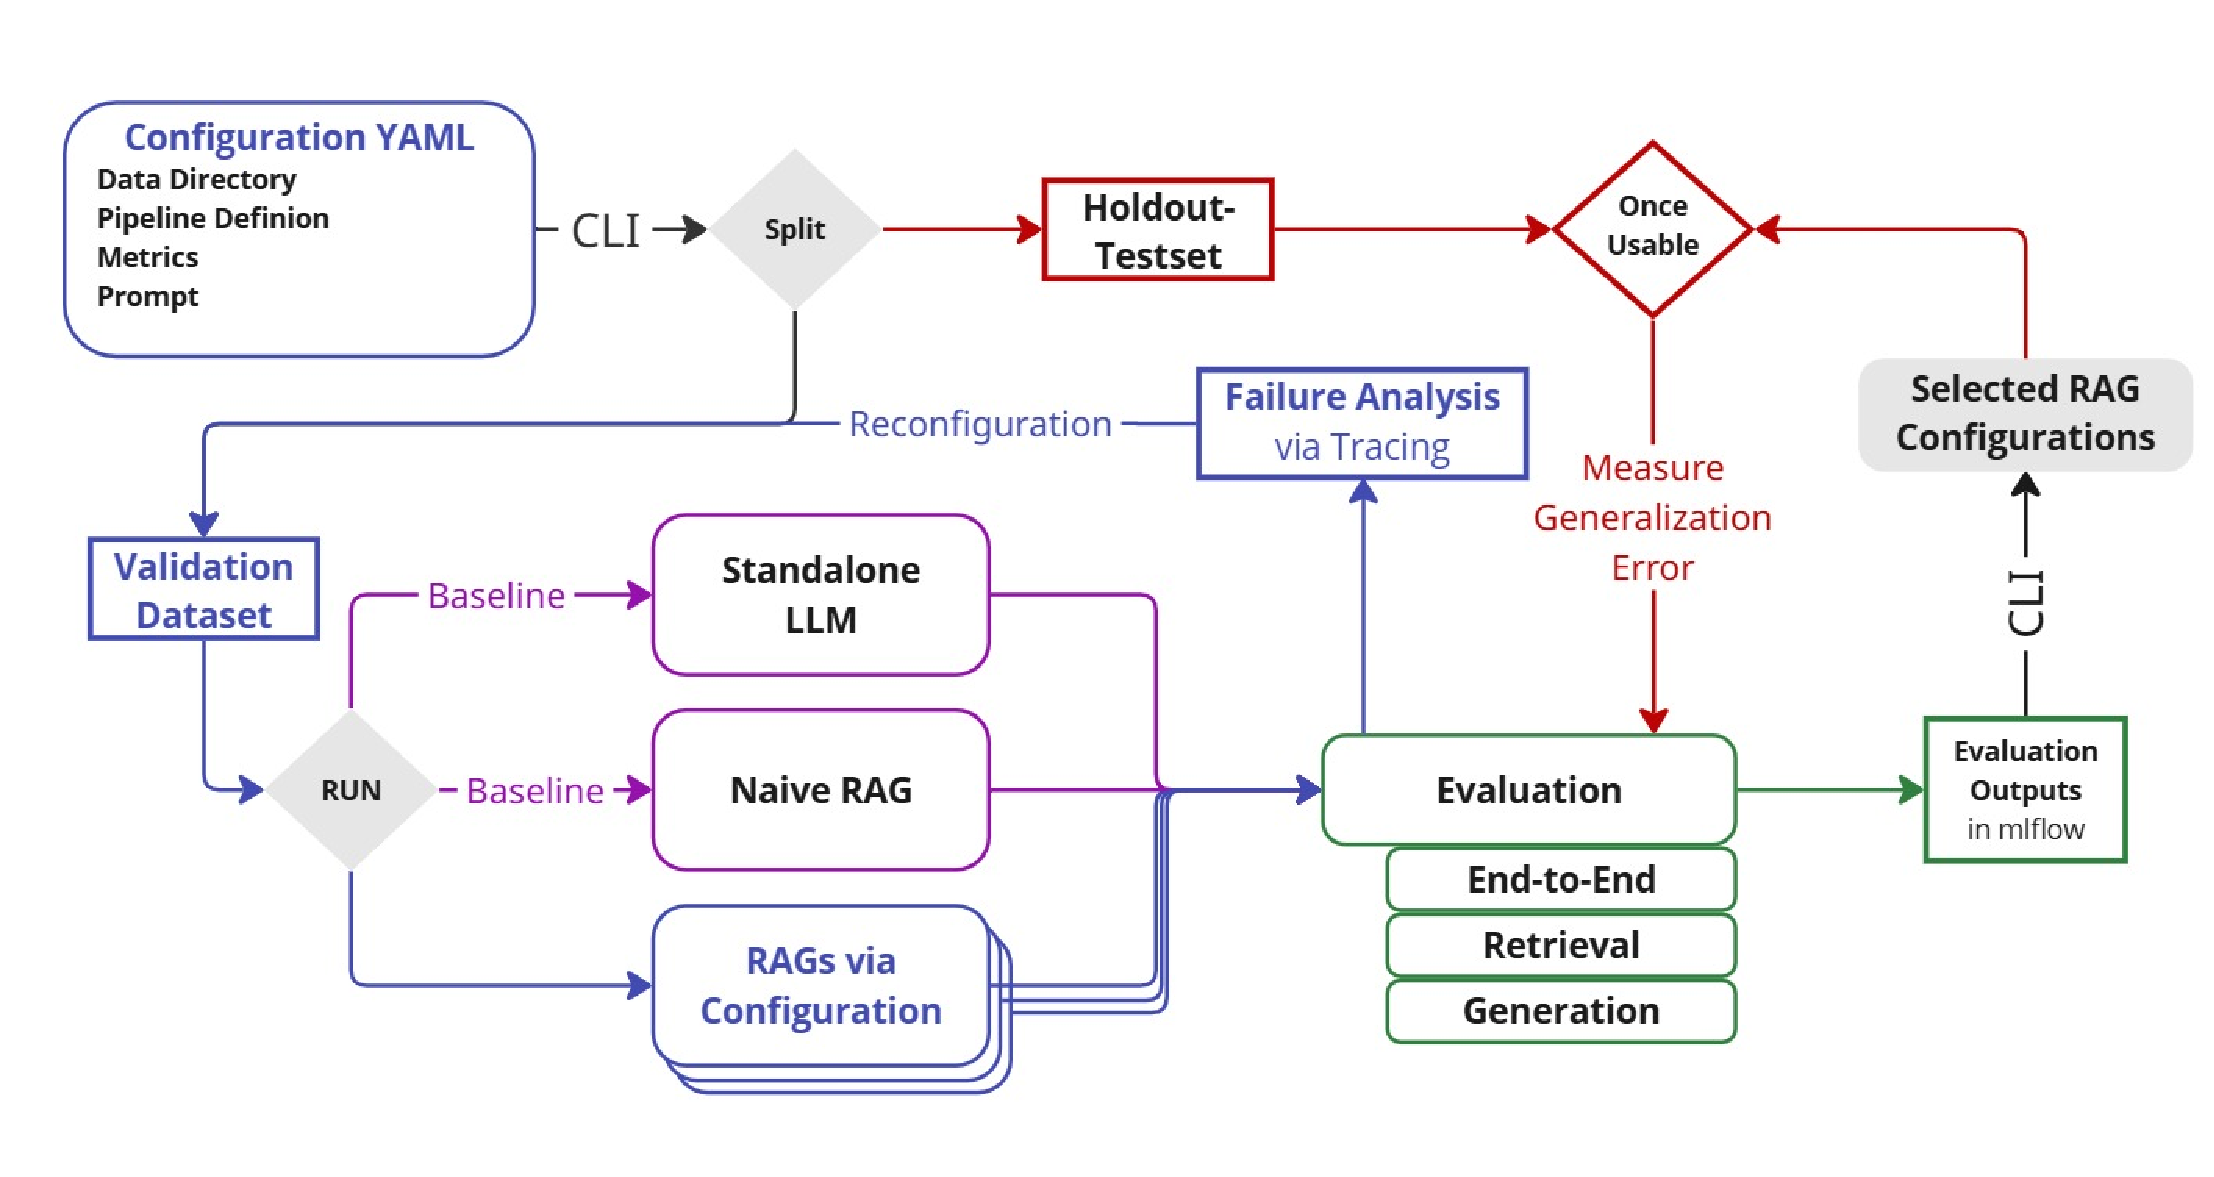
\includegraphics[width=\textwidth]{images/FrameworkFull.pdf}
  \caption{Framework: At first the evaluation data get splitted into validation and hold-out test dataset. Then the validation data is used to evaluate a configured RAG system and compare it against baselines. After failure analyisis several reconfiguration phases can happen. At last the test dataset is used to test all configurations for a potential generalization error.}
  \label{fig:framework-full}
\end{figure}


\section{Transparency}

We are following Simon et al.\cite{Simon.10112024} recommendations for ensuring transparency in RAG experiments. First we ensure that the used data is either publicly availlable or published by the experimenter. This does not fall under the functionality of this framework, because this is usually done via version control such as Github\cite{github-inc-2025} or Gitlab\cite{gitlab-inc-2025}. Another popular decision is DVC\cite{dvc.17.03.2025}, which is primarly focussed on machine learning experiments and therefore less suited for RAG development. Their approach of adding stages is a lot of overhead that might be too time-consuming for fast RAG development. Beside that derived features such as visualisation are adjusted to training which is epoch-oriented. 

Code as well as RAG-system architecture is saved with each commit. This ensures that every configuration phase can be restored as well as transparently reported. 

We added in all configuration files meta data parameters. We highly recommend this practice for every configuration phase. There can be written down comments, hypothesis or simple thoughts that can later on be used to compare different results within MLflow. Additional this can be used to make it more transparent why this reconfiguration phases were executed. This has several benefits.
At first, it makes researchers intentions more clear e. g. did the researcher wanted to improve retrieval or context utilization? 
Second, it also shows unsuccessful configurations or hypothesis, which can be used by other research teams later on.

Typical machine learning experiments require seeding, which can be complicated as it is not clear which services support it. We included it in the openai generators in our example configurations and want to raise attention for including seeding in all applicable situations.

The here stated transparency considerations and actions make sure that RAG experiments are reproducible as much as we can. It assumes a static dataset. If the dataset is frequently changing the users needs to use a workaround with DVC, which we have decided not to include.
Beside that all experiments are reproducible as long as all components of the system that include randomness can pass a seed parameter.

\section{Validity}

\paragraph{Internal Validity}
Evaluating semantics in LLM's or RAG systems rely on LLM-as-a-Judge models or lexical metrics such as BLEU or ROUGE, which measure the token overlap of actual answer and ground truth. Lexical answers can not capture answer pairs that are differently written but having the same semantic. LLM-as-a-Judge are on par with human-level judging, but are prone to preference leakage. There are findings suggesting that LLM-as-a-judge favor similar LLMs that their based on. Therefore using synthetic data for evaluation is fast, but risks preference leakage.\cite{Li.03.02.2025} This field is very new and still under research. We implemented our LLM-as-a-Judge metric for context utilization with environment variables that default to OpenAIs \textit{gpt-4o-mini}\cite{OpenAI_2022}. We warn users actively about this potential bias and let them have the possibility to vary the generator model family from the LLM-as-a-judge model family.

\begin{figure}
    \centering
    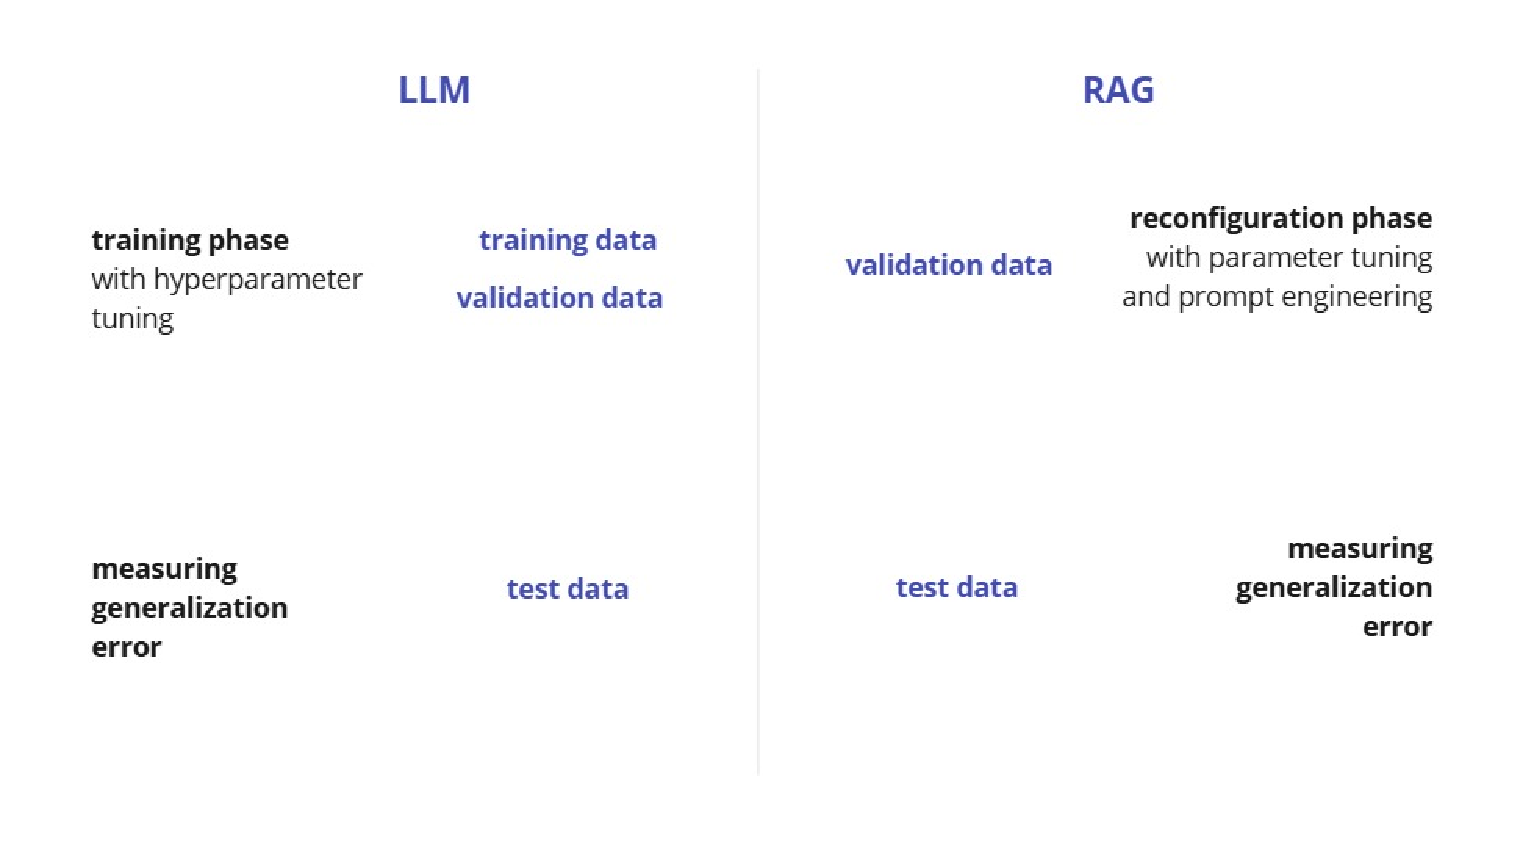
\includegraphics[width=\textwidth]{images/RAGvsLLM-tuning.pdf}
    \caption{Comparison of reconfiguration between RAGs and LLMs - both relying on tuning parameters and test data.}
    \label{fig:tuning}
\end{figure}

\paragraph{External Validity}

With our framework we handle one part of external validity concerns for RAG experimentation. We split the data into validation and test dataset so that all reconfiguration phases happen on the validation dataset, no matter if they include custom trained components or not. Only at the last stage of this development, the generalization error is estimated and the test dataset is used. Users can then compare per MLflow experiment run metrics calculated on validation data versus metrics calculated on test data. The visualisation should enlight which system configurations perform only on validation data well. 

\section{User Interface}

We use the presented Haystack functionalities to build a CLI-based framework around it. Our complete appraoch can be seen in figure \ref{fig:framework-full}. Given a data directory, pipeline and metrics definition, we first split the data into a validation and holdout-test dataset based on a split parameter \textit{test\_size}. Next we use the resulting validation dataset to run the first evaluations on the data. For that it loads the pipeline and data from its paths and starts with evaluating against a standalone LLM to have a baseline if RAG at all is a significant improvement in contrast to having just an LLM. Next, it ingests data into a vector database and builds an naive RAG with (Retrieve-Read) architecture as another baseline in contast to the in the YAML file defined advanced RAG architecture. The same procedure starts with the RAG configuration from the file. Each run gets evaluated in respect to End-to-End evaluation and component-wise. Evaluations are visualized in MLflow. Traces are shown in LangFuse. You can see both in the figures \ref{fig:mlflow} and \ref{fig:langfuse}. After failure analysis, the RAG can be reconfigured again to test new parameters. 

\begin{figure}
  \centering
  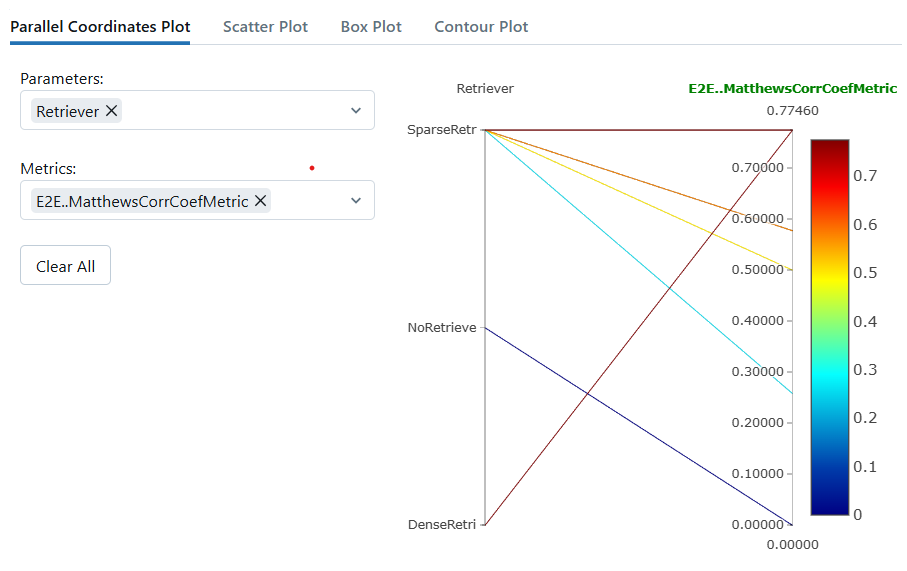
\includegraphics[width=\textwidth]{images/MLFlow-Vis.png}
  \caption{Example of a MLflow run in our framework. We can define different hypothesis, comments or similar via meta information in our configuration files. Then we can compare metrics based on those annotations.}
  \label{fig:mlflow}
\end{figure}

\begin{figure}
\centering
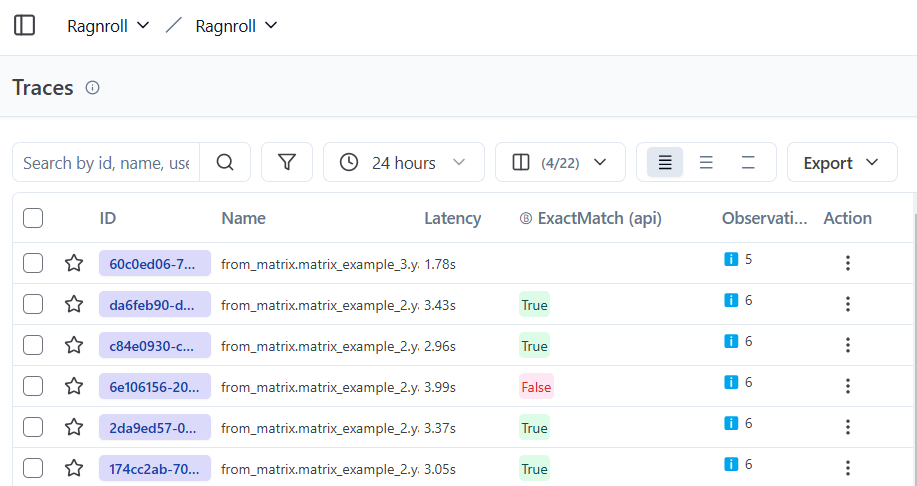
\includegraphics[width=\textwidth]{images/langfuse.png}
\caption{Example of a Langfuse instance. We always post for each trace if the system was successfully predicting the classification result so that users can find failures fast and efficiently.}
\label{fig:langfuse}
\end{figure}

The framework provides a command-line interface built with Typer that enables efficient RAG evaluation workflows. Two main commands are available: \textit{run-evaluations} executes experiments against baseline models (standalone LLM and naive BM25 RAG) and custom configurations defined in YAML files, with results logged to MLflow; and \textit{test-generalization-error} evaluates optimized configurations against the held-out test set. All commands integrate with Langfuse for tracing and MLflow for experiment tracking, ensuring reproducible and transparent RAG development.

\section{Limitations}

This Framework focusses primarly on classification tasks. However, the framework is expandable via custom metrics so that users could in theory define their own metrics classes for generalization tasks. 

We implemented the framework as modular as possible so that every possible architecture with all customized components can be evaluated. We can not guarantee that every architecture is possible and supporting agentic workflows might need further work.



% Some Explanatory Notes:
% Do I have to make a minimal manual here? I don't think so. I guess I have to write down What I have decided WHY

% Was unterscheidet mein Framework von existierenden?